\documentclass[twocolumn]{article}
\usepackage{calc}
\usepackage{ifthen}
\usepackage[margin=0.5in]{geometry}
\usepackage{amsmath,amsthm,amsfonts,amssymb}
\usepackage{amsfonts}
\usepackage{color,overpic}
\usepackage{hyperref}
\usepackage{array} 
\usepackage{amstext}
\usepackage{enumitem}
\usepackage{graphicx}
\usepackage{caption}
\usepackage{natbib}
\usepackage{framed}
\usepackage{float}
%\usepackage[]{algorithm2e}
\usepackage{algpseudocode} 
\usepackage{algorithmicx}
\usepackage{tabto}

\newenvironment{Figure}
  {\par\medskip\noindent\minipage{\linewidth}}
  {\endminipage\par\medskip}
  
\numberwithin{equation}{section}

\NumTabs{10}

% Turn off header and footer
\pagestyle{empty}
\setlist[itemize]{leftmargin=*} % set itemise indentation to leftmargin
\setlist[enumerate]{leftmargin=*}

\setlist[itemize]{itemsep=0mm}
\setlist[enumerate]{itemsep=0mm}

\title{Linear Algebra}
\date{\vspace{-6ex}}

% -----------------------------------------------------------------------

\begin{document}
\maketitle

\textbf{Linear algebra} is the branch of mathematics concerning vector spaces and linear mappings between such spaces.


\section{Basic Definition}

	\subsection{Matrix operation}
\begin{itemize}
	\item Addition: $(\mathbf{A} + \mathbf{B})_{i,j} = \mathbf{A}_{i,j} + \mathbf{B}_{i,j}$
	\item Scalar multiplication: $(c\mathbf{A})_{i,j} = c \cdot \mathbf{A}_{i,j}$
	\item Transposition: $(\mathbf{A}^\mathrm{T})_{i,j} = \mathbf{A}_{j,i}$
	\item Matrix multiplication: $ (\mathbf{AB})_{i,j} =\sum_{r=1}^n A_{i,r}B_{r,j},$
	\begin{itemize}
		\item Associative: 	$ \mathbf{(AB)C = A(BC)}$
		\item Distributive : $\mathbf{A}(\mathbf{B} + \mathbf{C}) = \mathbf{AB} + \mathbf{AC}$
		\item Not commutative: $\mathbf{A}\mathbf{B} \neq \mathbf{B}\mathbf{A}$
	\end{itemize}
\end{itemize}

	\subsection{Square Matrix}
A \textbf{square matrix} is a matrix with the same number of rows and columns.	
\begin{itemize}    
	\item Triangular: $\mathbf{U}_{i,j} = 0 \mbox{ if } i > j\ $ and  $\mathbf{L}_{i,j} = 0 \mbox{ if } i < j\ $
	\item Diagonal (up. and low. tri.): $\mathbf{D}_{i,j} = 0 \mbox{ if } i \ne j\ $
	\item Diagonalizable : $\mathbf{A | \exists P, P^{-1}AP=D} $ (diagonal)
	\item Identity (diag.) : $\mathbf{I}_{i,j} = \{0 \mbox{ if } i \ne j\ ; 1 \mbox{ if } i=j \} $
 	\item Symmetric matrix: $\mathbf{A} = \mathbf{A}^{\mathrm{T}} \mbox{ or } a_{i,j}=a_{j,i}$
 	\item Invertible: $\mathbf{A} \mid \exists \mathbf{A^{-1}} \mbox{ with }\mathbf{AA^{-1}} = \mathbf{A^{-1}A} = \mathbf{I}$
	\item Positive definite (sym.): $\mathbf{A} \mid \mathbf{x}^T\mathbf{A}\mathbf{x} > 0 \quad \forall \mathbf{x}\not=0 \in \mathbb{R}^n$
	\item Orthogonal matrix: $\mathbf{A}_{i,.}$ and $\mathbf{•}hbf{A}_{.,j}$ are orthonormal vectot. This is equivalent to say $\mathbf{A^\mathrm{T}}=\mathbf{A^{-1}}$ or $\mathbf{A^\mathrm{T}}\mathbf{A}=\mathbf{I}$
	\item Unitary matrix (complex analogue to orthogonal): $\mathbf{A}^* \mathbf{A} = \mathbf{A}\mathbf{A}^* = \mathbf{I} $
\end{itemize}


	\subsection{Main Operation}
\begin{itemize}
	\item Trace (square): $\operatorname{tr}(\mathbf{A}) = \sum_{i=1}^{n} \mathbf{A}_{i,i}$
	\item Determinant (square):  is a number encoding certain properties of the matrix.
	\item The rank of a matrix is the maximum number of linearly independent columns (or line) vectors of the matrix.
	\item Conjugate: $(\overline{\mathbf{A}})_{i,j}=\operatorname{Re}(\mathbf{A}_{i,j}) - \operatorname{Im}(\mathbf{A}_{i,j})$
	\item Conjugate transpose or Hermitian transpose: $\boldsymbol{A}^* = \boldsymbol{A}^H = \overline{\boldsymbol{A}}^\mathrm{T} = \overline{\boldsymbol{A}^\mathrm{T}}$
\end{itemize}	











\section{Other stuff}

	\subsection{Set, Field, Vector space, Span and Basis}
\begin{itemize}
	\item A \textit{set} is a collection of distinct or well defined objects, considered as an object in its own right
	\item A \textit{field} as a set together with two operations: addition  and multiplication (axiom: associativity, commutativity and distributivity hold). Futhermore, every nonezero element of F has an inverse such that $f^{-1} \times f=1$
	\item A \textit{vector space} over a field F is a set V together with two operations: addition and scalar multiplication (the same axiom hold). The difference is that the multiplication is between an element of F and V and not two element of V. Any field F is a vector space over itself and in this special case the two operations are similar.
	\item The \textit{kernel} (or nullspace) of a linear map $L : V \rightarrow W$, is the set of all elements v of V for which L(v) = 0. That is, in set-builder notation,
$$\ker(L) = \left\{ \mathbf{v}\in V | L(\mathbf{v})=\mathbf{0} \right\}$$
The difference of any two solutions $u$ and $v$ of the linear equation $\mathbf{Ax = b}$ lies in the kernel of A $(\mathbf{u}-\mathbf{v}) \in \ker(A)$:
$$ \mathbf{A(u-v)} = \mathbf{Au} - \mathbf{Av} = \mathbf{b} - \mathbf{b} = \mathbf{0} $$
\item  The \textit{linear span} of a set of vectors S in a vector space V is the intersection of all subspaces containing that set.
	\item A \textit{basis} is a set of vectors ($v_i$)in a vector space $V$ which are linearly independent (i.e. $\sum a_i v_i=0 \Rightarrow a_i=0$)and every other vector in the vector space is linearly dependent on these vectors (i.e. $x=\sum a_i v_i$).
	\item A \textit{orthonormal basis} is a basis which vectors ($e_i$) are orthogonal and have unit length (i.e. inner product null $ \langle e_i, e_j\rangle=0$ if $i\neq j$ and  $\langle e_i, e_i\rangle = \|e_i\| = 1$ )
	\item The \textit{support} of a function  is the set of points where the function is not zero-valued :$\operatorname{supp}(f) = \{x\in X \,|\, f(x)\ne 0\}$
	\item The \textit{frame} of a vector space V with an inner product (Hilbert space ?) can be seen as a generalization of the idea of a basis to sets which may be linearly dependent.
\end{itemize}


	\subsection{Linear dependence}
A set of n vectors $\mathbf{v}_i$ is said to be linearly dependent if one of the vectors $\mathbf{v}_k$ in the set can be defined as a linear combination of the other vectors.
$$\mathbf{v}_k=\sum_{i=0}^{n} a_i \mathbf{v}_i \quad \mbox{with } i \neq k$$
And therefore the set of vector is linear independent if the only representations of 0 as a linear combination of its vectors is the trivial representation:
$$ \sum_{i=0}^{n} a_i \mathbf{v}_i = 0 \Rightarrow \forall a_i=0 $$
\begin{itemize}
	\item n vectors in $\mathbb{R}^n$ are linearly independent if and only if the determinant of the matrix formed by taking the vectors as its columns is non-zero.
$$\det([\mathbf{v}_1,...\mathbf{v}_n])=0 \Leftrightarrow {\mathbf{v}_1,...\mathbf{v}_n} \mbox{ are linearly independant}$$
\end{itemize}




	\subsection{Eigenvalues and eigenvectors}
When viewing the square matrix A as a linear transformation, an \textbf{eigenvector} is a vector which direction is invariant under the transformation and which norm change by a scalar $\lambda$ called eigenvalue.
$$\mathbf{Av} = \lambda \mathbf{v}$$
This can be rewrite $\mathbf{Av} -\lambda \mathbf{v} = (\mathbf{A} -\lambda\mathbf{I}) \mathbf{v}=0$. Either the solution is $x=0$ in which case, the system would be inversible, be linearly indenpendant and has a none zero determinant. Either it is not the only solution, the system is singular and the determinant is equal to 0
$$\det(\mathbf{A} -\lambda\mathbf{I})=0$$


	\subsection{Inner Product}
The \textbf{inner Product} associates a scalar quantity ($\in F$) to each pair of vectors ($\in V$): $ \langle \cdot, \cdot \rangle : V \times V \to F $. It satisfies conjugate symmetry $\langle x,y\rangle =\overline{\langle y,x\rangle}$, linearity with first argument $\langle ax,y\rangle = a \langle x,y\rangle$ and positive-definiteness $\langle x,x\rangle \geq 0$.

\begin{itemize}
	\item The inner product generalized the \textbf{dot product} in euclidean space:
	$\mathbf{A}\cdot \mathbf{B} = \|\mathbf A\|\,\|\mathbf B\|\cos\theta = \sum_{i=1}^n A_iB_i $ 
	\item \textbf{Orthogonality} is define by a inner product null
	\item \textbf{Norm} is define as the inner product of the vector itself
\end{itemize}

We say that two non-zero vectors u and v are \textbf{conjugate} (with respect to A) if and only if they are orthogonal with respect to this inner product:
$$  \langle \mathbf{u},\mathbf{v} \rangle_\mathbf{A}=\mathbf{u}^\mathrm{T} \mathbf{A} \mathbf{v} = 0 $$

	\subsection{Complete Space}
A metric space M is called complete if every Cauchy sequence (sequence whose elements become arbitrarily close to each other as the sequence progresses) of points in M has a limit that is also in M or, alternatively, if every Cauchy sequence in M converges in M.

	\subsection{Projection}
In the general definition a projection is a linear transformation P from a vector space to itself such that P$^2$ = P (idempotent). In a Hilbert space with the inner product, the orthogonal projection can be used

The projection of two vector can be written as
	$$\mathrm{proj}_{\mathbf{u}}\,(\mathbf{v}) = {\langle \mathbf{u}, \mathbf{v}\rangle\over\langle \mathbf{u}, \mathbf{u}\rangle}\mathbf{u} =\frac{\mathbf{u} \mathbf{u}^\mathrm{T} }{\mathbf{u}^\mathrm{T} \mathbf{u}} \mathbf{v} = \mathbf{P} \mathbf{v} $$
\begin{figure}[H]
\centering
    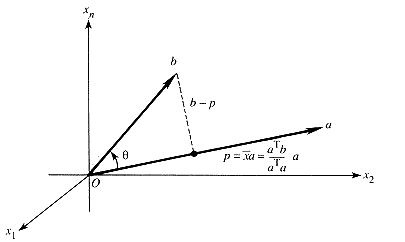
\includegraphics[width=.30\textwidth]{projection1.png}
\end{figure}

The projection $\mathbf{p}$ of a vector $\mathbf{b}$ into a subspace $\mathbf{A}=[\mathbf{a}_1,...\mathbf{a}_n]$ must have the error $\mathbf{b-p}$ perpendicular to the subspace
$$\mathbf{A^\mathrm{T}(b-p)}=0=\mathbf{A^\mathrm{T}(b-Ax)} \Rightarrow \mathbf{x= (A^\mathrm{T}A)^{-1}A^\mathrm{T}b}$$
and,
$$\mathbf{p=Ax=A(A^\mathrm{T}A)^{-1}A^\mathrm{T}b}$$

Where $P=Ax=A(A^\mathrm{T}A)^{-1}A^\mathrm{T}$ is the projection matrix.

	\subsection{Gram-Schmidt Process}
The Gram-Schmidt process is a method for orthonormalising a basis. It takes a finite, linearly independent set ${v_1, \ldots, v_k}$ and generates an orthonormal set ${e_1, ..., e_k}$.
$$ \mathbf{u}_k  = \mathbf{v}_k-\sum_{j=1}^{k-1}\mathrm{proj}_{\mathbf{u}_j}\,(\mathbf{v}_k) \qquad \mathbf{e}_k = {\mathbf{u}_k\over \|\mathbf{u}_k \|}.
$$
\begin{figure}[H]
\centering
    
\includegraphics[width=.30\textwidth]{GramSchmidtprocess.png}
\end{figure}
Numerical stability can be improve with the stabilized Gram-Schmidt
\begin{framed}\begin{algorithmic}
\State $i\gets 1$
\While{$i<k$}
	\State $\mathbf{v}_i \gets \frac{\mathbf{v}_i}{\|\mathbf{v}_i\|}$  \Comment{normalize}
	\State $j\gets i$
	\For{$j<k+1$}
		\State $ \mathbf{v}_j \leftarrow \mathbf{v}_j - \mathrm{proj}_{\mathbf{v}_{i}} \, (\mathbf{v}_j)$  \Comment{remove component in direction $v_i$}
		\State $j\gets j+1$
	\EndFor
\State $i\gets i+1$
\EndWhile
\end{algorithmic}\end{framed}


	\subsection{Inversion}
A square matrix $\mathbf{A}$ is \textbf{invertible} if it exist $\mathbf{A}^{-1}$ such that $\mathbf{AA^{-1}} = \mathbf{A^{-1}A} = \mathbf{I}$
It is equivalent to say:
\begin{itemize}
	\item The columns of $\mathbf{A}$ are linearly independent.
	\item A has full rank; $\operatorname{rank}(\mathbf{A}) = \dim(\mathbf{A})$.
	\item $\det(\mathbf{A}) \neq 0$
	\item Solution of $\mathbf{Ax=b}$ is unique
	\item The only solution of $\mathbf{Ax=0}$ is $\mathbf{x}=0$
\end{itemize}
A not invertible matrix is called singular
	

	\subsection{Generalized and pseudo inverse}
A \textbf{generalized inverse} of a matrix A is a matrix that has some properties of the inverse matrix of A but not necessarily all of them:
\begin{enumerate}
\item generalized inverse  $AA^{\mathrm g}A = A$ 
\item $A^g$ is a weak inverse $A^{\mathrm g}AA^{\mathrm g}= A^{\mathrm g}$
\item $AA^g$ is Hermitian   $(AA^{\mathrm g})^{\mathrm T} = AA^{\mathrm g}$
\item $A^gA$ is Hermitian  $(A^{\mathrm g}A)^{\mathrm T} = A^{\mathrm g}A $
\end{enumerate} 
If it satisfies all 4 conditions, then it is a Moore-Penrose pseudoinverse. 
Some properties:
\begin{itemize}
	\item The pseudoinverse exists and is unique for any matrix $A$.
	\item If $A$ is invertible, its pseudoinverse is its inverse $A^+=A^{-1}$.
	\item The pseudoinverse of the pseudoinverse is the original matrix: $(A^+)^+=A$
\end{itemize} 



	\subsection{Positive-Define Matrix}
Any quadratic function can be written as $f(\mathbf{z})=\mathbf{z^\mathrm{T}Mz}$. The meaning of a positive define matrix, is one which the function associated has a unique minimum zero when $\mathbf{z}=0$ and strictly positive otherwise and is strictly convex.

The following properties are equivalent to A, a symmetric square matrix being positive definite:
\begin{itemize}
	\item $x^TAx>0 \quad \forall x\neq 0 \in$
	\item All its eigenvalues are positive.
	\item all these determinants are positive
\end{itemize}




	
\section{Matrix decomposition}
A matrix decomposition is a factorization of a matrix into a product of matrices.

	\subsection{Decompositions related to solving systems of linear equations}
		\subsubsection{LU factorization}
of a square matrix $\mathbf{A}$ is into a lower L and upper U triangular matrix $\mathbf{A = LU}$ 
	
		\subsubsection{QR factorization } 
of a matrix $\mathbf{A}$ with linear independent vector is into a product $\mathbf{A = QR}$ of an orthogonal ($\mathbf{Q^TQ=I}$) matrix $\mathbf{Q}$ and an upper triangular matrix $\mathbf{R}$ (or U). The orthonogal matrix can be produce with the Gram-schmidt algorithm (transforming linear independent vector in orthonormal one)
	
		\subsubsection{Cholesky decomposition} 
of a square, symmetric, positive definite matrix $\mathbf{A}$ into upper triangular with positive diagonal entries and its transporse $\mathbf{A=U^TU}$

	\subsection{Decompositions based on eigenvalues and related concepts}
		\subsubsection{Eigendecomposition}
of a square matrix $\mathbf{A}$ with distinct eigenvectors into a square matrix $\mathbf{Q}$ whose column is the eigenvector of $\mathbf{A}$ and adiagonal matrix $\mathbf{\Lambda}$  whose diagonal elements are the corresponding eigenvalues.
	$$\mathbf{A}=\mathbf{Q}\mathbf{\Lambda}\mathbf{Q}^{-1}  $$

		\subsubsection{Takagi's factorization}
of a square, complex, symmetric matrix A into a diagonal matrix and a unitary and its transpose. 
$$ A=VDV^T$$
This is the special case of the eigendecomposition where $A$ is real-symmetric and therfore $V$ is invertible $V^T=V^{-1}$.
The geometrical interpretation is a rotation $V^T$, a scaling $D$ and the back-rotation transform $V$

	
		\subsubsection{Singular Value Decomposition}	
SVD of an m$\times$n complex matrix $M$ is a factorization of the form:
$$\mathbf{M} = \mathbf{U} \boldsymbol{\Sigma} \mathbf{V}^*$$
where $ \mathbf{U}$ is unitary, $\boldsymbol{\Sigma}$ is diagonal and $\mathbf{V}^*$ is the conjugate transpose of an unitary matrix $\mathbf{V}$. The diagonal entries $\sigma_i$ of $\mathbf{\Sigma}$ are known as the singular values of $\mathbf{M}$.

Like the eigendecomposition below, SVD involves finding basis directions along which matrix multiplication is equivalent to scalar multiplication, but it has greater generality since the matrix under consideration need not be square.

In the case of square matrix with positive determinant, SVD  can be interpreted as a composition of : a rotation ($\mathbf{V}^*$), a scaling ($\mathbf{\Sigma}$), and another rotation ($\mathbf{U}$).

\begin{figure}[H]
\centering
    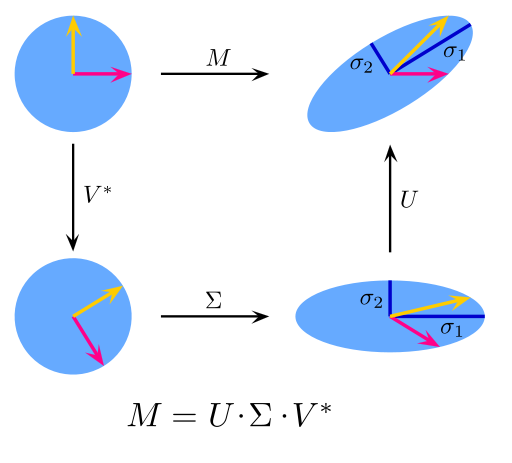
\includegraphics[width=.30\textwidth]{512px-Singular-Value-Decomposition.png}
\end{figure}





\bibliographystyle{apalike}
\bibliography{citations}	
	

\end{document}
